\begin{frame}
\frametitle{Pauli's neutrino}
\begin{columns}
\column{0.45\textwidth}
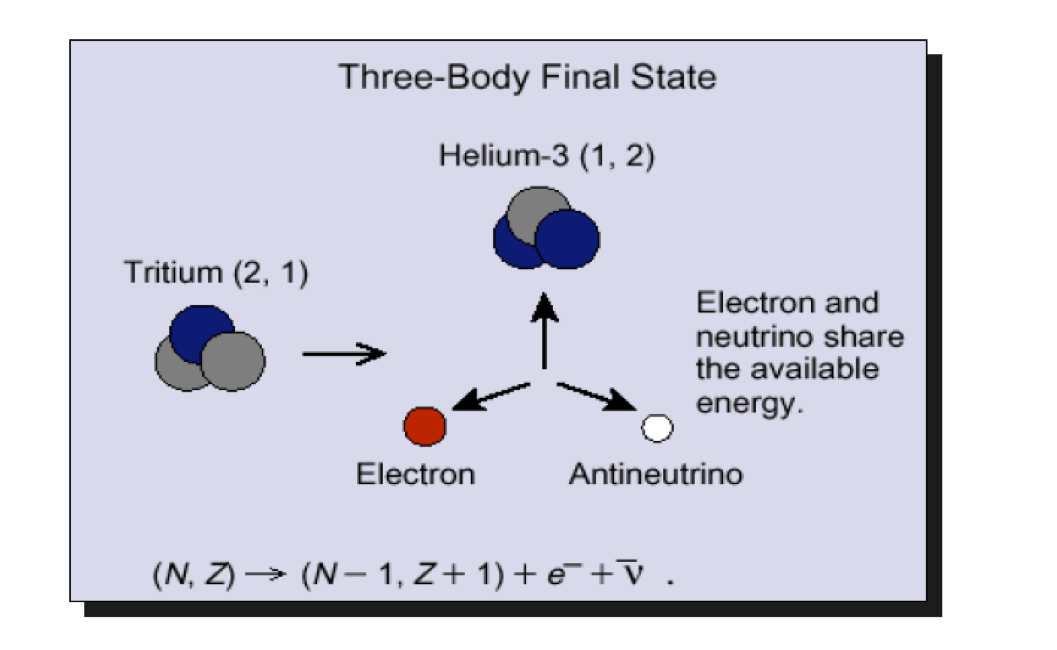
\includegraphics[scale=0.4]{pauli-neutrino.png}
 
 \column{0.3\textwidth}
\begin{block}{}
{\bf Electrically neutral particles which have spin 1/2 and obey the exclusion principle... the mass should be of the order of the electron mass}. In other words, Pauli ``neutrons''  were nothing but neutral electrons. 
\end{block}
\end{columns}
\end{frame}
